\chapter{Discussion}\label{sec:discussion}
\section{Rayleigh Scattering Slope}
\paragraph{HAT-P-12b}
For HAT-P-12b, we use additional high precision data from \cite{Sing2016}\footnote{Data downloaded from http://www.astro.ex.ac.uk/people/sing/spectra/?/people/sing/spectra/HAT-P-12b} using HST/STIS in the optical wavelengths (see \S \ref{sec:followup}). As shown in Fig.~\ref{fig:hatp12_sing}, the measured Rp/Rs (black) in MuSCAT g-,r-,and z-bands are superposed with the data (magenta) and atmospheric model (green line) of \cite{Sing2016}. Fitting our measurement with this model yields a $\chi^2$/ d.o.f.= 0.316 implying overestimated uncertainties. %This confirms that the observed trend is consistent with the previous result.
%Using HST data alone, $\chi^2$/dof=0.998
%Using HST+MuSCAT data, $\chi^2$/dof=0.950
Although our achieved (1 $\sigma$) uncertainties for Rp/Rs are only about 2$\times$ to 5$\times$ to that in \cite{Sing2016}, we note that that our results for HAT-P-12b cannot conclusively distinguish between our two atmospheric models. To distinguish between our two models however, we only need an improvement 1.5$\times$ photometric precision in g-band.
This is because the 1$\sigma$ fractional uncertainties of the measured Rp/Rs is at the level of $\sim$2 times as large as one scale height (See Table~\ref{tab:H/u}). In the case of HST/STIS observations, the fractional uncertainties %$H/\sigma_{Rp/Rs}$ 
are between 0.5-2.2 scale heights in the optical wavelengths.
In any case, this confirms the validity of our transit modeling approach that %correctly measured the predicted radius variation of HAT-P-12b at the wavelengths relevant for our observation. 
produce measurements that do not significantly deviate from the theoretical Rayleigh slope.
%can also be interpreted as consistent with a flat spectrum without the knowledge of the published HST/STIS spectra. 

%\paragraph{HAT-P-44b}

\begin{figure}
\centering
	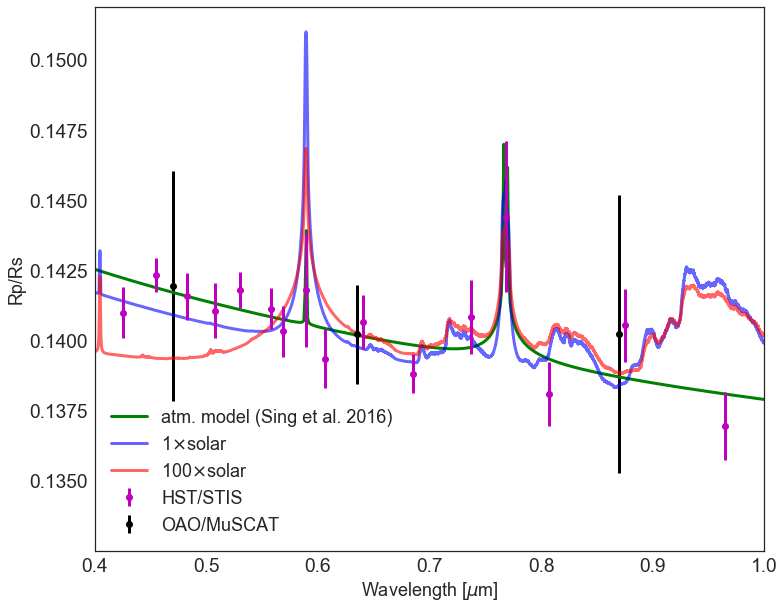
\includegraphics[width=10cm]{hatp12/atm_model_full.png}
    \caption{Transmission spectrum of HAT-P-12b. The measured Rp/Rs using MuSCAT in g-,r-,and z-bands (red points) are superposed with the data (blue points) and atmospheric model (green line) of \cite{Sing2016}. The vertical lines represent 1-$\sigma$ uncertainties.
    }\label{fig:hatp12_sing}
\end{figure}

\paragraph{WASP-21b}
As shown in Table~\ref{tab:wasp21_map}, we found a %mean variation 
difference of $\sim$0.3\%  in the transit depth of WASP-21b %09670, 0.09889, 0.09998
between z- and g-bands which is greater than the uncertainties. 
As opposed to Rayleigh scattering feature (negative slope) in the optical wavelength, the apparent trend (positive slope) is inconsistent with our atmospheric model. 
%Archival data of WASP-21b\footnote{http://var2.astro.cz/ETD/etd.php?STARNAME=HAT-P-21&PLANET=b} show a transit depth variability semi-amplitude of at most 7 mmag in R-band. %and 5 mmag in clear band.  
To confirm that this feature is inherent in the data and not due to our modeling, we re-analyze each light curve independently. We show in Fig.~\ref{fig:wasp21_combined_grz} that the result is consistent with increasing transit depths towards shorter wavelengths. 

As stellar activity can affect the measurement of a transmission spectrum, we %photometrically monitored 
check the activity levels of WASP-21 by analyzing archival data from ETD.\footnote{} 
WASP-21 shows low levels of stellar activity, with observed photometric variations or upper limits which are sufficiently small that their effects on measuring the transmission spectra are minimal compared to the measurement errors3,4,11–13. %We try to were corrected for occulted and un-occulted star spots10,14. 
We reserve the discussion of the nature of this trend in \S \ref{sec:spots}.

\begin{figure}
\centering
	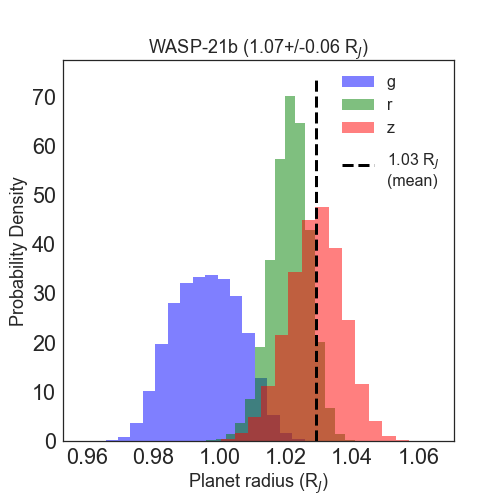
\includegraphics[width=8cm]{wasp21/radius_ratios_Rjup_per_band.png}
    \caption{Posterior distribution of Rp/Rs obtained from independent (i.e. per color) re-analysis of WASP-21 light curve showing trend consistent with simultaneous, multi-color modeling.}
    \label{fig:wasp21_combined_grz}
\end{figure}

%Finally, we search for Rp/Rs variations with wavelength, which can in principle be observed due to the atmospheric opacity variations. %The measured Rp/Rs values and their uncertainties in respective bands are listed in Table 6 and shown in Figure 6. 
%A constant fit to these values gives the mean value of Rp/Rs = 0.08179  0.00064 with c2 = 13.0 for dof=6, meaning that Rp/Rs is constant over the observed wavelength range within 2$\sigma$. 

\section{Significance of Detection}
%In the following, we aim to determine whether the measured Rp/Rs in all bands are constant or consistent with a Rayleigh slope over the observed wavelength range. 
To evaluate the robustness of our detection, we did a Monte Carlo simulation in which we sample from the posterior distribution of Rp/Rs of each band and computed the Rayleigh slope. The distribution of slope and intercept are shown in Fig.~\ref{fig:hatp12_slope}--Fig.~\ref{fig:wasp21_slope}. The dashed red and blue line correspond to Rayleigh scattering slope expected for 1 Solar and 100 Solar atmosphere model, respectively. The mean of the slope distribution is biased away from the dotted black line by at least 1$\sigma$. In other words, all the data set cannot be explained by a flat spectrum. Even though both HAT-P-12b and HAT-P-44b spectra is consistent with a Rayleigh slope in the optical, our detections are marginal. 
%Equivalently, the mean of the slope distribution is consistent with the predicted theoretical Rayleigh slopes. 
However, the measured uncertainty (width of the slope distribution) is not small enough to distinguish between two atmospheric models as also evident in the model spectra.

Following \cite{Fukui2016a}, we estimate how sensitive these Rp/Rs measurements are to atmospheric signatures by comparing the estimated 1-$\sigma$ measurement error of Rp/Rs, $\sigma_{Rp/Rs}$, with the expected variation
of Rp/Rs due to the atmospheric effect. When a planet has an atmosphere with no thick clouds, Rp/Rs can vary with wavelength by up to several H/Rs. Therefore, if $\sigma_{Rp/Rs}$ is comparable to or smaller than the expected value of H/Rs, it can roughly be considered that the measurement is sensitive to the atmosphere. Based on Fig.~\ref{fig:HRs-sigRpRs}, our achieved precision is enough to detect atmospheric features but only for the case of WASP-21b.

\begin{figure}
\centering
	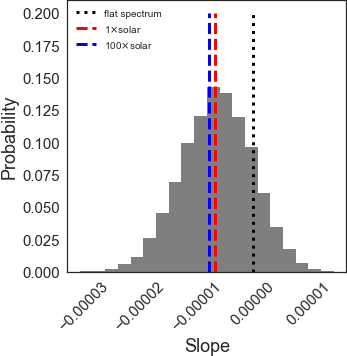
\includegraphics[width=8cm]{hatp12/slope.png}
    \caption{Monte Carlo simulation of fitting a straight line to the measured Rp/Rs by directly sampling from the posterior distribution. The red and blue vertical lines correspond to the expected slope for a 1$\times$ and 100$\times$ Solar atmosphere while the black line correspond to zero slope (i.e. flat spectrum). The mean slope is consistent with the expected Rayleigh slope and biased away from zero within 1.8$\sigma$.
    }\label{fig:hatp12_slope}
\end{figure}

\begin{figure}
\centering
	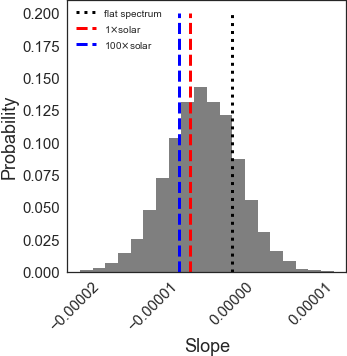
\includegraphics[width=8cm]{hatp44/slope.png}
    \caption{Same as in \ref{fig:hatp12_slope} but for HAT-P-P-12b. The mean slope is biased away from zero by 1.0$\sigma$.
    }\label{fig:hatp44_slope}
\end{figure}

\begin{figure}
\centering
	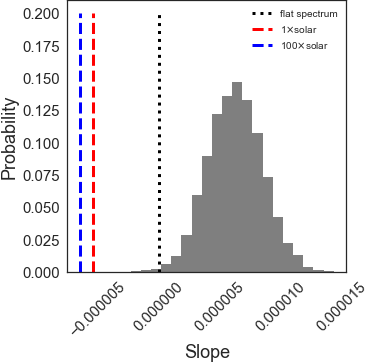
\includegraphics[width=8cm]{wasp21/slope.png}
    \caption{Same as in \ref{fig:hatp12_slope} but for WASP-21b. A positive slope is cannot be attributed to Rayleigh scattering. The mean slope is biased away from zero by 2.8$\sigma$.
    }\label{fig:wasp21_slope}
\end{figure}

\begin{table}
\centering
\caption{Required improvement in photometric precision to be sensitive to atmospheric features (See also Fig.~\ref{fig:HRs-sigRpRs}). Only z-band of WASP-21b is sensitive to detection of expected atmospheric feature.}
\begin{tabular}{lll}
\label{tab:H/u}
                  & & $\sigma_{Rp/Rs}/H/Rs$ \\ \hline                     
 \multirow{3}{*}{HAT-P-12b}& g-band:& 1.96 $\pm$ 0.19  \\
                           & r-band:& 1.44 $\pm$ 0.14  \\
                           & z-band:& 2.73 $\pm$ 0.26  \\ \hline
 \multirow{3}{*}{HAT-P-44b}& g-band:& 1.93 $\pm$ 0.06  \\
                           & r-band:& 1.80 $\pm$ 0.05  \\
                           & z-band:& 2.67 $\pm$ 0.08  \\ \hline
 \multirow{3}{*}{WASP-21b} & g-band:& 1.22 $\pm$ 0.06  \\
                           & r-band:& 1.05 $\pm$ 0.05   \\
                           & z-band:& 0.97 $\pm$ 0.05  \\
\hline
\end{tabular}
\end{table}

\begin{figure}
\centering
	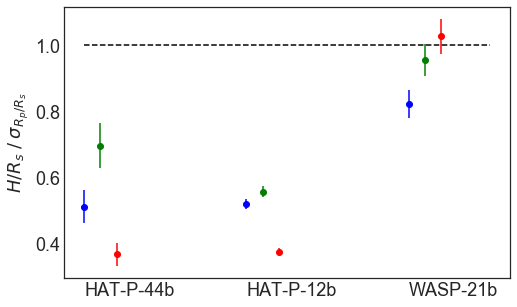
\includegraphics[width=10cm]{figures/H-sigRpRs.png}
    \caption{Measured sensitivity of Rp/Rs measurements to atmospheric signatures. $\sigma_{Rp/Rs}/H/Rs$>1 implies robust detection.}\label{fig:HRs-sigRpRs}
\end{figure}

%Note that optical and infrared data are both crucial for this claim of "cloudiness" because the measurement of a Rayleigh signal in the optical alone is not sufficient as it could be simply caused by H2 and He. Only a spectral slope less negative than −4 in the optical may allow us to infer the presence of large particle (a$\geq \lambda/2 \pi$) clouds from the spectrum alone, but this requires an accurate estimate of the atmospheric scale height (Heng 2016).

%In order to further explore the notion that the combination of individual light curves does tend to cancel out systematic errors present in the original data we have created Allan variance plots of the residuals (observed minus model) corresponding to each of the individual light curves and the residuals corresponding to the resulting combined light curves. For this, we followed the formalism detailed in Carter et al. (2009). We have used their definition of Allan variance as stated in their Equation (8) to plot its value as a function of lag. This is shown

\section{The Case of WASP-21b: Unocculted Star Spot} \label{sec:spots}
%However, best-fit model does not show apparent difference in transit depth among different filters. Is it because of sampling only? No! I checked that samples do show difference.
The apparent increase in transit depth towards longer wavelengths is not consistent with an atmospheric model including Rayleigh scattering in the optical as shown in Fig.~\ref{fig:atm_wasp21b}. Instead, this trend is consistent with unocculted starspots that may be present on the surface of the star but are not along the transit chord (i.e. different from a spot-crossing event e.g. \cite{Pont2008}). %unocculted spots mimic Rayleigh scattering in transmission spectrum (McCullough+2014; Oshagh+2014)
%After taking into account the overall flux level of the star and implementing a wavelength-dependent radius correction assuming a reasonable spot temperature, Pont+2008 and Sing+2011 attribute this effect to be of atmospheric origin and not stellar spots

Unocculted starspots are known to cause a systematic effect on the apparent Rp/Rs due to chromatic abberations and rotational modulations (see e.g., Carter et al. 2011; Désert et al. 2011b; Sing et al. 2011). 
These unocculted spots can be accounted for by a wavelength-dependent depth correction. As with \cite{Narita2013}, %Kirk+2016, 
we follow the formalism of \cite{Sing2011} to make this correction. %We use \verb'ATLAS9' stellar models (\cite{Kurucz1993}) of a star with temperature $T_{star}$ = 5800 K for WASP-21 and spot temperatures with temperature difference $\Delta T$ ranging from 250 K to 1250 K. Using this variation, we assume a total dimming 0.4\% at reference wavelength of 600 nm and use equations (4) and (5) in \cite{Sing2011} to find the correction in Rp/Rs across the wavelength range spanned by MuSCAT g- and z-bands (400-920 nm). %We find that the effect of spots on this star is large as they lead to a correction in Rp/Rs of between X and X which is comparable to the 1-sigma error bars of our measured Rp/Rs in MuSCAT data.
The systematic difference of the radius ratio $\Delta(R_p/R_s)$ caused by the stellar variability due to starspots can be written as
\begin{equation}
 \Delta(R_p/R_s) \simeq 0.5 \Delta f(\lambda) R_p/R_s
\end{equation}
where  $\Delta f(\lambda)$ is the stellar brightness variability at wavelength $\lambda$. 
Assuming the black-body profile for the emission from those regions, we search for an optimal spot coverage that can explain the semi-amplitude of g- and z-band variability. We find that a spot coverage of 0.5\% gives the best-fit for those two bands. This shows that our atmospheric modeling is useful to categorically rule out the possibility that the observed trend in WASP-21b spectrum is atmospheric in origin. 


\section{Selecting Future Targets for MuSCAT \label{sec:targetselection}}
The amplitude of the absorption within the exoplanet's atmosphere can be approximated as (e.g. \cite{Encrenaz2014})
\begin{equation}
A=10\frac{H}{R_s}\frac{R_p}{R_s}
\end{equation}

Thus, the critical property of a target when performing transit spectroscopy is the relative size of the planet to its star. This makes the atmospheres of large gas giants generally much easier to recover. Similarly, smaller planets around dwarf hosts are favorable. %55 Cnc e (Demory et al. 2011; Winn et al. 2011; V=5.95) and HD 97658b (Dragomir et al. 2013; V=7.7). 
However, only very few of these small targets are bright enough for atmospheric characterization from the ground. 

Table~\ref{tab:A} shows currently known targets with host brighter than m$_v$=13.5 and ranked in increasing amplitude for a Jovian, Neptunian, and terran-type exoplanet. At the time of writing, a few new targets joined the list including WASP-107, WASP-127 and EPIC 220674823/K2-106 which are being considered for proposal for MuSCAT. 

\begin{table}
\centering
\caption{Short-list of top 5 Jovian, Neptunian, and Terran transiting system ranked in decreasing $A$ signature.} 
\begin{tabular}{llllllll}
hostname	&	Vmag	&	$R_p$	&	$T_{eq}$	&	$R_s$	&	$T_{eff}$	&	$A [\%]$& Status	\\ 
\hline
Jovian (0.5 <R [R$_J$]<13)\\
\hline 
WASP-107	&	11.471	&	0.94	&	770	&	0.66	&	4430	&	0.103605	 & Proposed\\
WASP-17	&	11.6	&	1.991	&	1771	&	1.57	&	6650	&	0.098804	&  well-known\\
WASP-127	&	10.15	&	1.37	&	1400	&	1.39	&	5620	&	0.087652	& candidate \\
WASP-52	&	12	&	1.27	&	1315	&	0.79	&	5000	&	0.079451	& well-known \\
WASP-79	&	10.1	&	2.09	&	1900	&	1.53	&	6600	&	0.069718	& well-known \\ 
\hline
Neptunian	(0.35 <R [R$_J$]<0.5)	\\
\hline
K2-32	&	12.31	&	0.458	&	817	&	0.84	&	5275	&	0.018146	& candidate \\
HAT-P-11	&	9.472	&	0.422	&	878	&	0.75	&	4780	&	0.012263	& well-known \\
K2-27	&	12.64	&	0.4	&	902	&	0.89	&	5248	&	0.006348	& candidate \\
KOI-94/ Kepler-89	&	12.205	&	0.385	&	1012	&	1.52	&	6182	&	0.00432	& well-known \\
Kepler-4	&	12.7	&	0.357	&	1650	&	1.49	&	5857	&	0.003719	& well-known\\
\hline
Terran (R$_p$[R$_J$]<0.35) \\
\hline
GJ 1132	&	13.49	&	0.128	&	644	&	0.26	&	-	&	0.032978	& well-known \\
Kepler-78	&	11.551	&	0.105	&	2250	&	0.74	&	5058	&	0.006713	& well-known \\
EPIC 220674823/ K2-106	&	12.102	&	0.247	&	722	&	0.95	&	5496	&	0.005693	& well-known\\
K2-18	&	13.496	&	0.212	&	235	&	0.41	&	3457	&	0.004505	& well-known \\
Kepler-36	&	11.866	&	0.328	&	928	&	1.63	&	5911	&	0.010561	& well-known\\
\hline
\label{tab:A}
\end{tabular}
\end{table}

%To accurately detect wavelength dependent radius variation as a proxy for detecting Rayleigh scattering feature, however, photometric precision must achieve at least equal to the order of $H/R_s$.

%Because of the degeneracy between planets with high mean molecular weight atmosphere and those with high-altitude clouds or hazes %Miller-Ricci et al. 2009; Kreidberg et al. 2014) 
%optical transmission spectrum with Rayleigh scattering feature should be complemented with infrared spectrum. In such a case, observing a flat spectrum in the infrared proves that Rayleigh scattering feature detected in the optical constrains the existence of high-altitude clouds or hazes in the atmosphere.

\begin{comment}
estimates of S/N ratio for an 8 m telescope. The SINFONI/VLT time calculator is used in the K band, with an exposure time of 3 h and a resolving power of 4000. Note that the time calculator only takes into account the photon noise and assumes a perfect stability of the instrument and atmosphere, which is an optimistic assumption.

For a hydrogen-helium (H-He)-rich planet with $\mu$=2.4, the scale height can be expressed as
\begin{equation}
H=3.46\frac{T}{g}
\end{equation}
in metric units. The (surface) gravity $g$ can be expressed as
\begin{equation}
g=25\frac{M_p}{R^2_p}
\end{equation}
where $M_P$ and $R_P$ are the mass and the radius of the planet, expressed in Jovian masses and radii, respectively. Thus, the amplitude of the absorption can be written as
\begin{equation}
A=1.4\times 10^{-6}\frac{HR_p}{R^2_s}
\end{equation}
For hot Jupiters, typical values of $A$ are a few 10$^{-4}$. $A$ signature is especially strong for planets having a high temperature (and thus being close to their stars), a large radius and a low molecular weight. Inflated hot Jupiters are thus privileged targets for primary transits.
%Infrared spectroscopy of exoplanets: observational constraints
\end{comment}



\begin{comment}
%To accurately detect wavelength dependent radius variation as a proxy for detecting Rayleigh scattering feature, we search for transiting systems that have the lowest $H/R_s$. 
To select future targets amenable for future atmospheric characterization with MuSCAT, we compute $H/R_s$ for all known transiting exoplanets with well known $R_p$ and $R_s$. As seen in Eq\ref{eq:H}, scale height is a function of equilibrium temperature of the planet which is usually unknown a priori.
%First, we download the data available from NASA Exoplanet Archive \footnote{ https://exoplanetarchive.ipac.caltech.edu }. 
To estimate $H$ we first calculate the equilibrium surface temperature $T_{eq}(a,d)$ and surface gravity, $g_p(R_p,M_p)$ of the planet whenever empirical values are unavailable, and assume a fiducial mean molecular weight of $\mu$ = 2.3 for H-He dominated atmospheres. %The computed $H/R_s$ are summarized in Table~XX.%\ref{tab:future_targets}.
The plot is shown in Fig.~\ref{fig:future.png}.



%Fukui+2014a

The detectability of planetary atmospheric features through
the transmission spectrophotometry depends on how precisely
the Rp Rs value can be measured with respect to the expected
atmospheric scale height of the planet. For planning future
observations with MuSCAT, it is worthwhile investigating
what types of planet can be targeted by this instrument for the
atmospheric study.

To this end, we simulate the achievable measurement error
of Rp Rs with MuSCAT for planets with a range of sizes
around three types of host stars: 

the V = 10 F-dwarf HAT-P-14, 
the nearby (38 pc) K-dwarf HAT-P-11 (Bakos et al. 2010), and 
the nearby (14 pc) M-dwarf GJ1214 (Charbonneau et al. 2009). 

The properties of the respective stars are listed in Table 7. 

Spec. Type F5V K4V M4.5V
Radius (R) 1.59 0.683 0.211
Teff (K) 6600 4780 3026
Distance (pc) 205 38 14.3
g¢ 10.18 9.97a 15.58b
r¢ 9.94 9.16a 14.08b
z¢ 10.30 8.79a 11.86b


In each case we simulate that the host star has the
same size and brightness with the assumed star. The simulation
procedure is as follows. First we create a mock OOT light
curve for each star and each band from the residual light curve
in the same band of HAT-P-14b (see Figure 2). For mock OOT
light curves of HAT-P-14 we use the residual light curves as
they are. On the other hand, for HAT-P-11 and GJ1214 we
assume that all the conditions except for the brightness of the
host star (scintillation noise, photon noises from comparison
stars, sky background noise, and systematic noises) are the
same as those in the case of HAT-P-14, and set the error bar of
each data point in the mock OOT light curve by modifying the
error bar in the residual light curve as

\begin{figure}
\centering
	\includegraphics[width=7cm]{figures/future.png}
    \caption{Feasible targets amenable for .}
\label{fig:hatp12_tdv}
\end{figure}
\end{comment}








